\documentclass[a4paper]{report}
\usepackage[utf8]{inputenc}
\usepackage{graphicx}
\usepackage{titlesec}
\usepackage{float}

\titleformat{\chapter}[block]
    {\normalfont\huge\bfseries}{}{0pt}{\Huge}
\titlespacing*{\chapter}{0pt}{-40pt}{20pt}

\title{PRJ3-TrafficLight-SRS}
\author{ Group 7 }
\date{November 2021}

\begin{document}

\maketitle
\newpage
\tableofcontents

\chapter{Introduction}

\section{Purpose}
The purpose of this document is to specify the general scope and requirements for an advanced traffic light control system. This system is used by the Traffic Control International Inc. The target markets for this system are Germany and the Netherlands.

\section{Scope}
The scope of this project is to develop a system to control different types of traffic lights. It shall be able to switch the traffic lights depending from other traffic lights as well as pedestrian lights. This should be displayed in text for presentation and later in a simple GUI.

\section{References}
[1]  IEEE  Software  Engineering  Standards  Committee,  “IEEE  Std  830-1998,IEEE Recommended Practice for Software Requirements Specifications”, June25, 1998

\section{Definitions, acronyms, and abbreviations}
In this document are the following acronyms, and abbreviations used:\\\\
\begin{tabular}{|l|l|}
    \hline
    \bf Term & \bf Definition\\
    \hline
    fig. & figure/diagram \\
    \hline
    etc. & et cetera\\
    \hline
\end{tabular}\\

\section{Overview}
The following document describes the general specifications for the app and the web-interface. It is structured as follows: 
\begin{itemize}
    \item Chapter 1: Introduction\\
    This section is a general introduction to this document and the usage of it.
    \item Chapter 2: Overall description\\
    This section gives a general overview of the requirements of the application.
    \item Chapter 3: Advanced information\\
    This section describes the requirements given in the previous section in detail.
\end{itemize}

\newpage
\chapter{Overall description}

\section{Product perspective}
The product stands alone and shall be implemented as a whole system. A simple text display should be implemented to display the full functionality of the product. At later updates of the system a simple GUI for display of functionality shall be added as well. All functionalities shall be available for all users of the system.

\section{Product functions}
The major features of the traffic light system are displayed in the use case diagram below (fig. \ref{fig:useCaseDiagram}):\\\\
\begin{figure}[H]
    \centering
    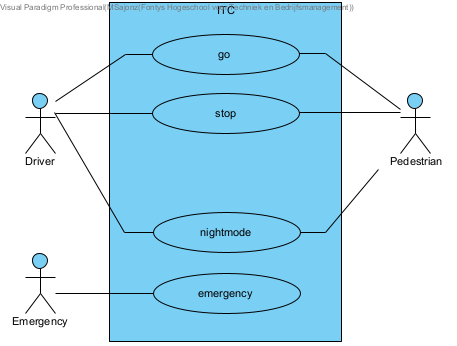
\includegraphics[scale=0.75]{Use_case_diagram}
    \caption{use case diagram}
    \label{fig:useCaseDiagram}
\end{figure}

\begin{figure}
    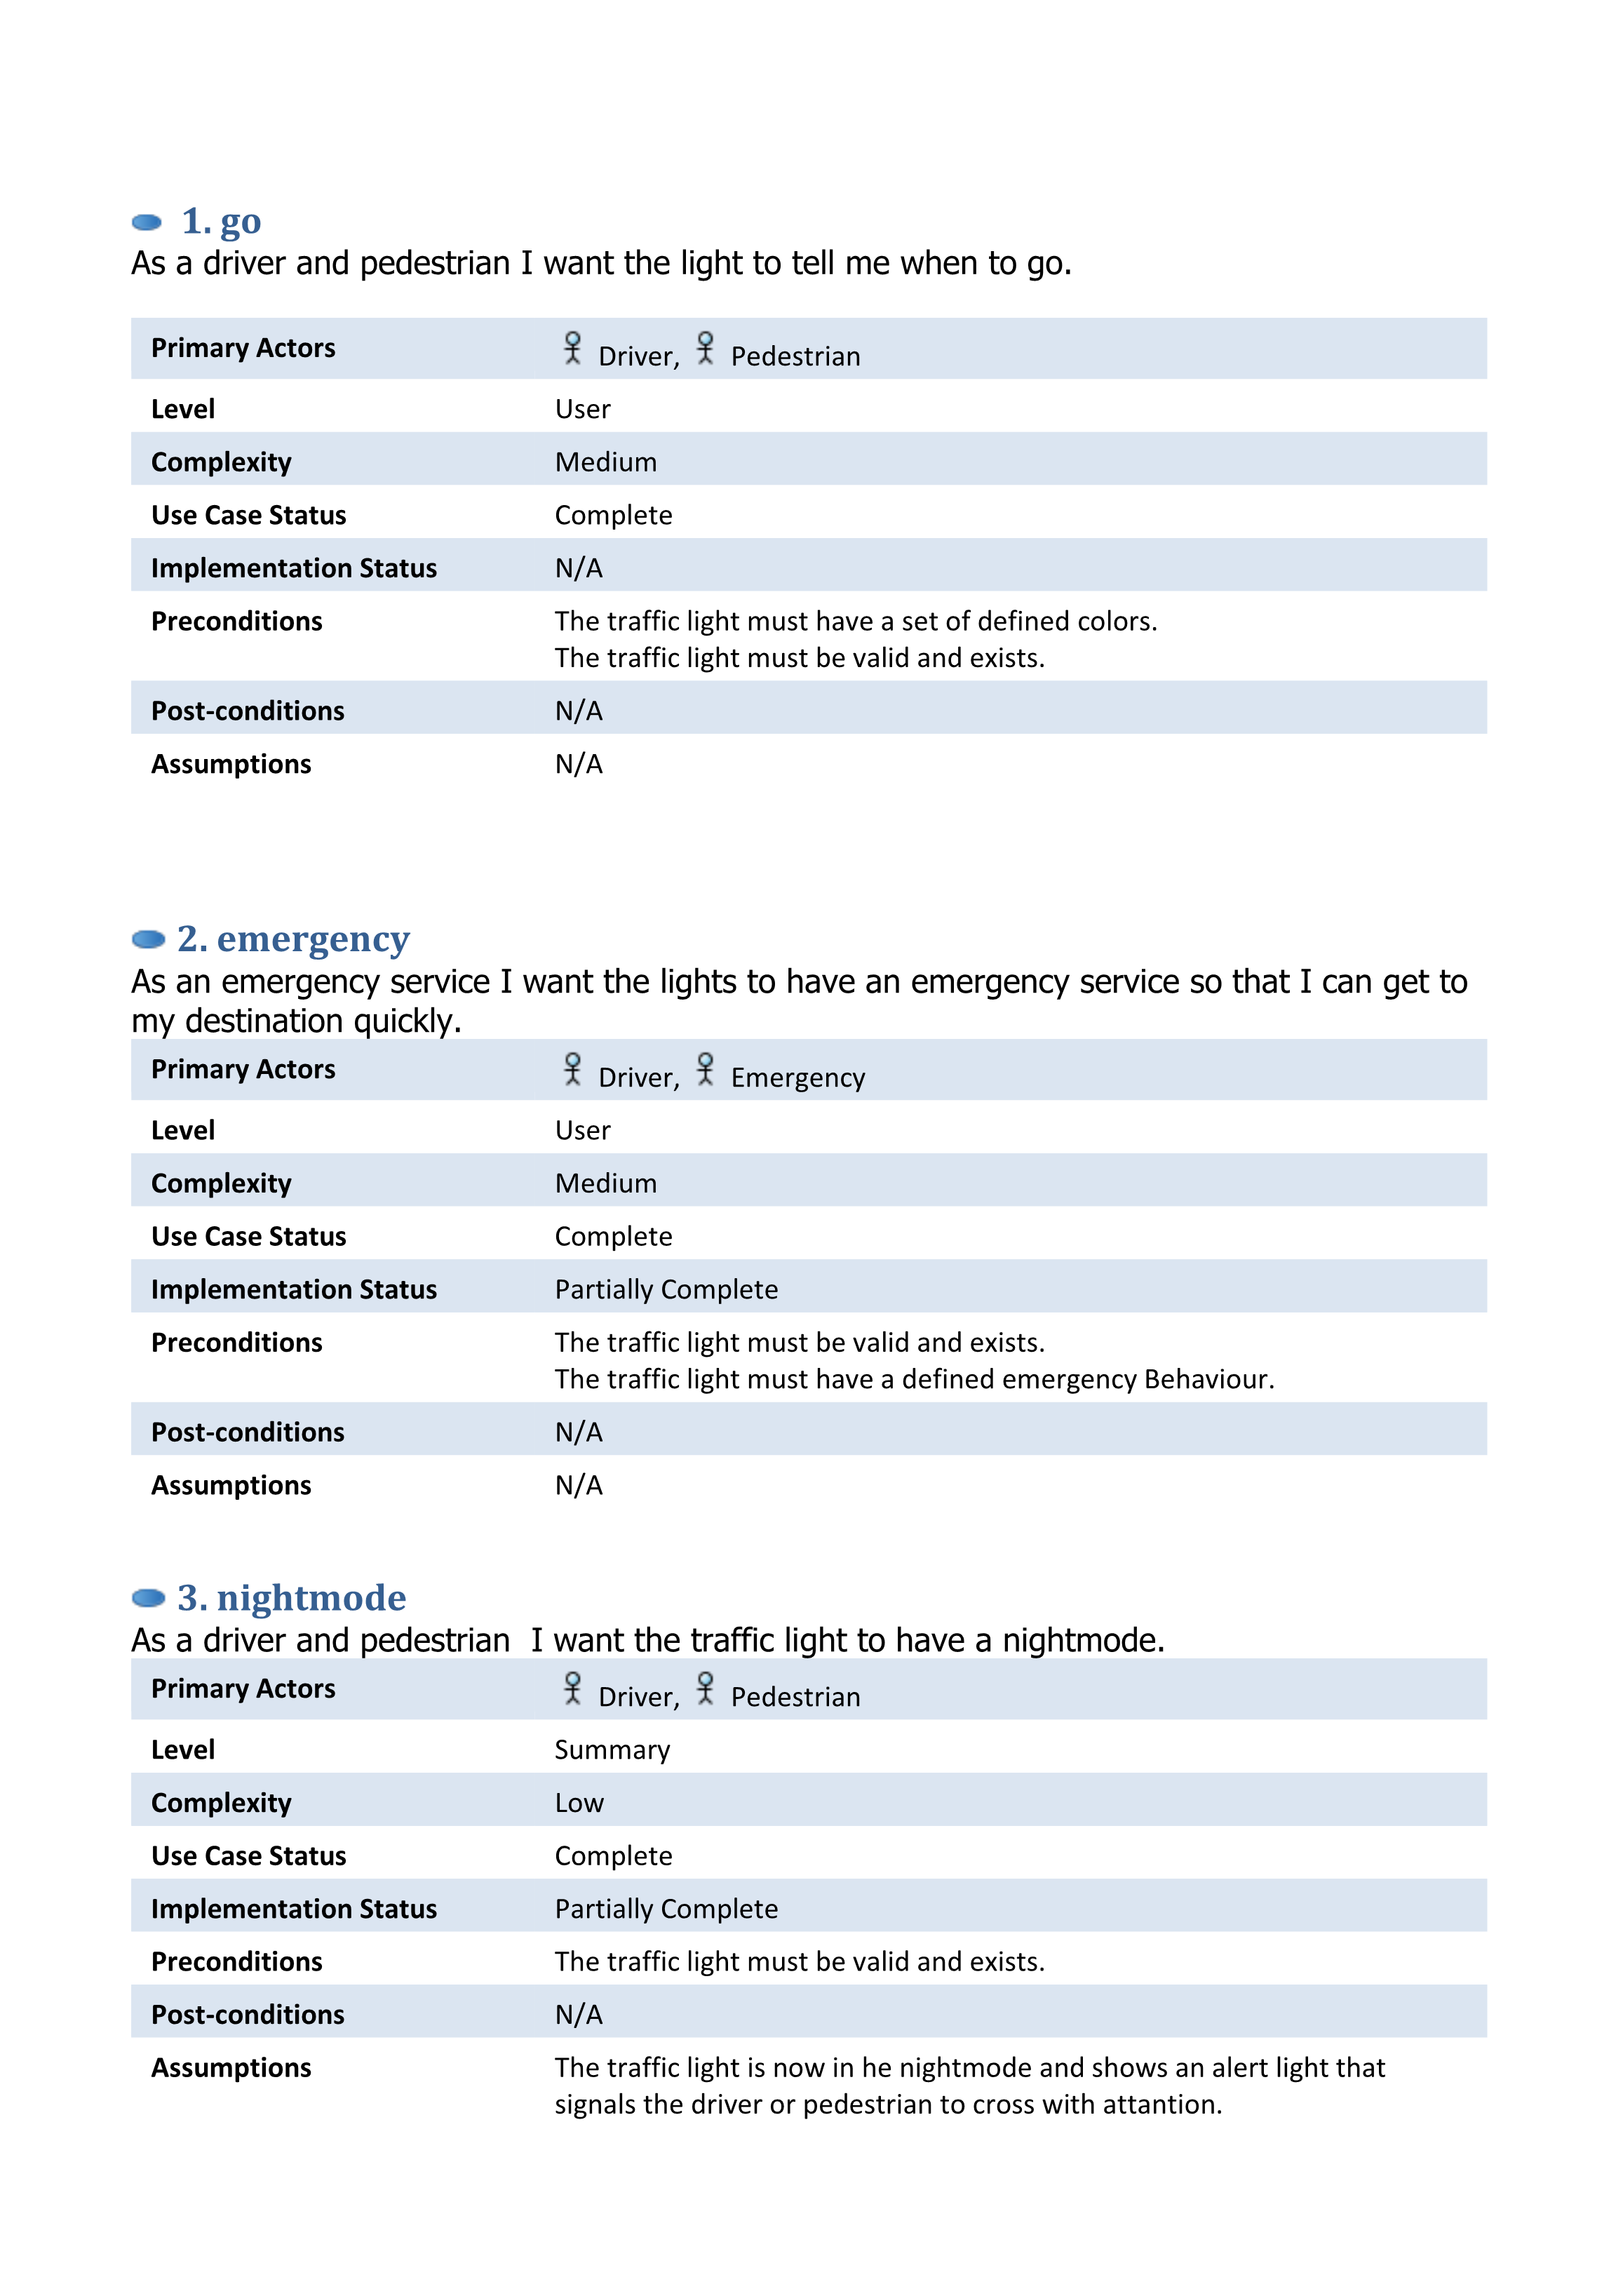
\includegraphics[scale=0.75]{p2}
    \caption{Requirement Specification 1}
    \label{fig:requSpec1}
\end{figure}

\begin{figure}
    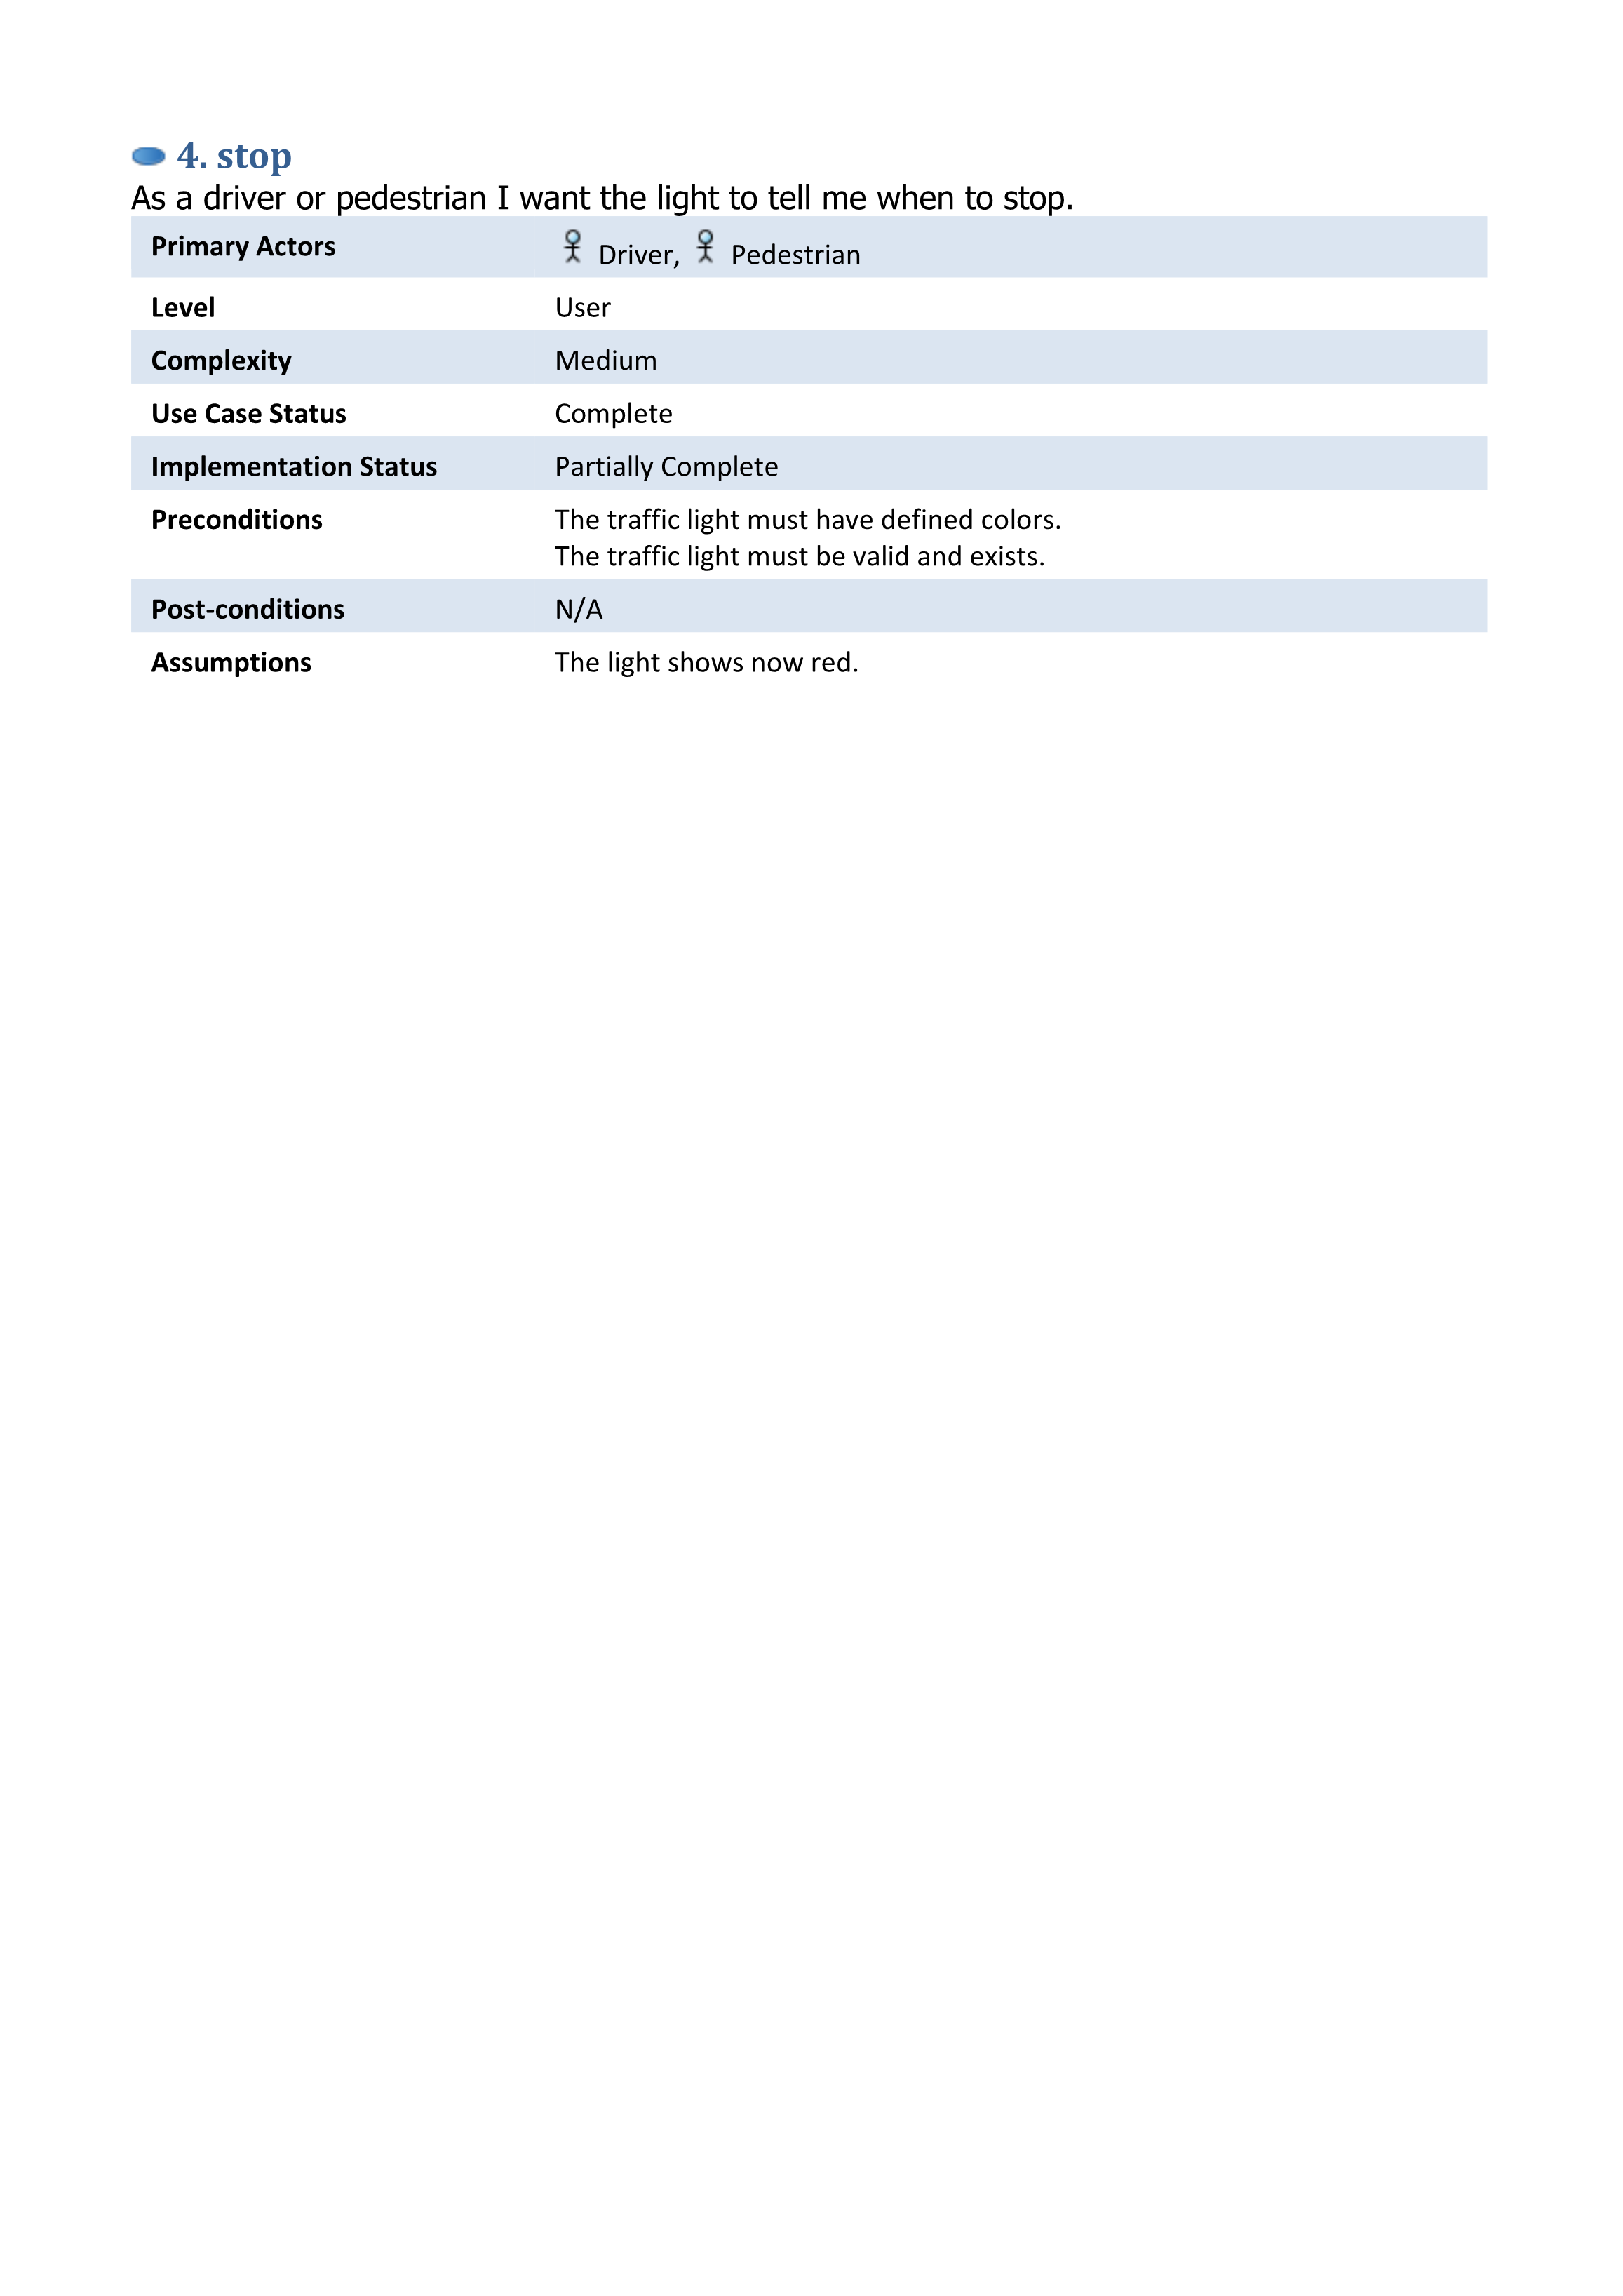
\includegraphics[scale=0.75]{p3}
    \caption{Requirement Specification 2}
    \label{fig:requSpec2}
\end{figure}

\newpage
\section{User Characteristics}
Users of the system shall only be employees of the company which maintains the traffic lights and uses the system for controlling them. The system should be designed to allow all types of users the access without high knowledge of technologies.\\\\
Available functions:
\begin{itemize}
    \item change traffic light colors
    \item change pedestrian light colors
    \item change traffic lights dependent on other traffic lights as well as pedestrian lights
    \item change light behavior dependent on the location of the traffic lights
    \item enable emergency mode for emergency services
\end{itemize}

\section{Constraints}
\begin{itemize}
    \item at a crossing the traffic light should turn red when the pedestrian light turns green
    \item if the traffic light turns green the pedestrian light shall turn red
\end{itemize}
These constraints are applicable for all types of crossings like 4 way crossing or 2 way crossings.

\section{Assumption and dependencies}
For using the application a device with decent specifications is required to run the GUI. For the text only a device with low specifications is required. The application does not need an internet connection. For real life usage are traffic lights as well as pedestrian lights required.

\chapter{Specific requirements}

\section{Functions}
In this section are the main functionalities of this system described.
Mainly the system shall be able to control different types of traffic lights. These are a normal traffic light for cars and pedestrian traffic lights. These lights shall be able to change its color dependent from the other. These lights shall have the standard light colors and shapes of the country where they are placed. For Germany for example are red, yellow and green required. The behaviour for a normal traffic light is different in every country. This should be adaptable as well as the color and the shapes. The light behaviour for Germany is for example green, yellow, red. If the start color is red the behaviour changes. The behaviour is now red, red-yellow, green. This does not count for the pedestrian light. These are different in every country as well as their color and shape behaviour.

\section{Design constraints}
The application shall not require any other hardware than the device used by the user or the traffic lights if executed on a real life example. 

\section{Software system attributes}
The following section describes attributes of the software that should be maintained as a guideline for implementation. 

\subsection{Reliability}
If input data is given by the user it shall be checked to secure the expected functionality of the system.

\subsection{Availability}
The system shall start at user request and shall run independent from user input. The start phase shall be defined. On this start phase should all other colors be directed.

\subsection{Maintainability}
The system shall not require to be maintained. Once implemented the system shall be easily adaptable even if the system is transferred to another country.

\subsection{Portability}
The system shall run on MacOS as well as on Windows devices. 

\section{Organization the specific requirements}
The main feature which shall be implemented is that the traffic light are able to change its color. Based on this feature all other features shall be implemented. First the text based interface shall be finished. If there is time left at the end of main feature implementation there should be a graphical user interface designed.

\end{document}
